\newpage
\section{Multiplexing}\label{sec:multiplexing}
Okay, we've covered how data gets transmitted over a medium and how we can modulate signals to represent our data. That's cool! Unfortunately, with the busy lives we lead, we need lots of data - fast! So, how do we cram all this data into our limited bandwidth? Enter multiplexing!

Multiplexing is the technique of combining multiple signals into one signal over a shared medium. This allows us to make the most out of our available bandwidth by sending multiple data streams simultaneously. It's exactly like the MUXes you've already seen in Computer Architecture, but now we're applying it to the physical layer of networking.

\subsection{Time Division Multiplexing (TDM)}
\label{subsec:tdm}
Time Division Multiplexing (TDM) shares a single link by slicing time into fixed-length slots. Each source is assigned one slot per frame; sources take turns in a periodic round-robin\footnote{
    Round robin is a scheduling algorithm where each source gets a fixed time slice in a cyclic order. 
}, so only one transmits at any instant and there is no mutual interference. If a source has nothing to send, its slot may be left idle (synchronous TDM) or reallocated on demand (statistical TDM).

\begin{figure}[h]
    \centering
    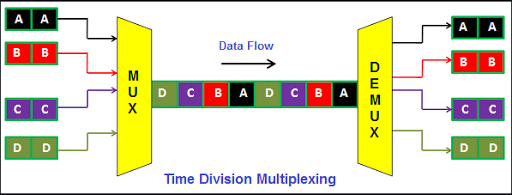
\includegraphics[width=.8\textwidth]{assets/osi/physical/multiplexing/tdm.png}
    \caption{Time Division Multiplexing (TDM) example}
    \label{fig:tdm_example}
\end{figure}

\subsection{Frequency Division Multiplexing (FDM)}
\label{subsec:fdm}
Frequency Division Multiplexing (FDM) divides the available bandwidth into non-overlapping frequency bands, each carrying a separate signal. Each source is assigned a unique frequency band, allowing multiple signals to be transmitted simultaneously without interference.

\subsection{Wavelength Division Multiplexing (WDM)}
\label{subsec:wdm}

Wavelength Division Multiplexing (WDM) is a specialized form of FDM used in fiber optic communication. It allows multiple optical signals to be transmitted simultaneously over a single fiber by using different wavelengths (colors) of light. This significantly increases the capacity of the fiber, enabling high-speed data transmission over long distances.


\subsection{Multiple Access}
You might come across the term "multiple access" in networking. Especially in this course. Recall that multiplexing is about sharing a medium among multiple signals (i.e. data streams), which can be thought of as a single device (or two, in the case of communication), sending multiple signals at once towards each other.

\begin{importantblock}
    Multiple access, on the other hand, is about how \textbf{multiple devices} share a medium to communicate with each other.
\end{importantblock}

\subsection{Code Division Multiple Access (CDMA)}
\label{subsec:cdma}
Code Division Multiple Access (CDMA) allows multiple signals to share the same frequency band simultaneously. CDMA uses unique code sequences called "chip codes" to distinguish between different users' signals.

\paragraph{How Chip Codes Work}


Each transmitter receives a unique binary sequence (chip code) with these properties:
\begin{itemize}
    \item Much longer than data bits (typically 64-128 chips per bit)
    \item Mathematically orthogonal to other users' codes
    \item Produces strong correlation when multiplied by itself
    \item Produces near-zero correlation with different codes
\end{itemize}

When sending data, each bit is multiplied by the entire chip code. The receiver recovers the original data by multiplying the received signal with the same code and integrating over the bit period.


\begin{figure}[h]
    \centering
    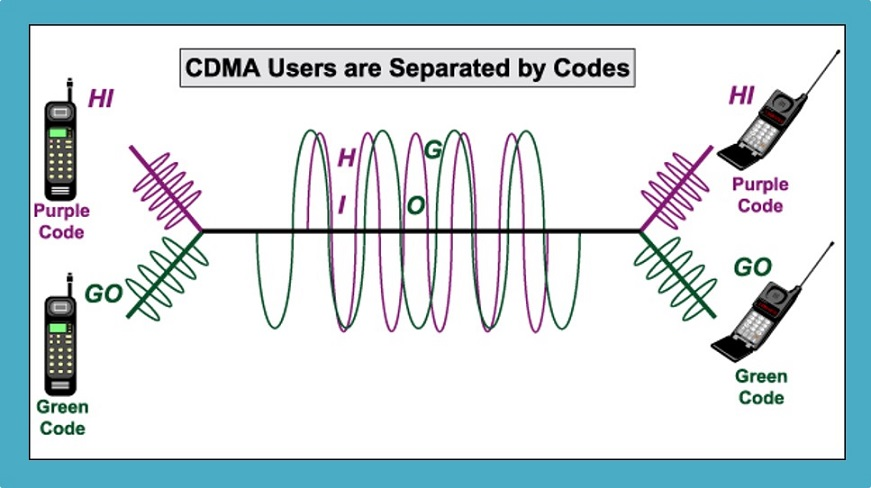
\includegraphics[width=0.7\textwidth]{assets/osi/physical/multiplexing/cdma_example.png}
    \caption{CDMA encoding showing how data bits are spread using chip codes}
    \label{fig:cdma_example}
\end{figure}


\subsubsection{Orthogonality of Chip Codes $\star$}

CDMA deals with the problem of multiple users transmitting simultaneously. We can make the analogy with multiple people talking over each other: if everyone speaks over each other, it's a mess. But if the group involved is comprise of pairs of people, each speaking their own, completely different language, they can communicate without interference (because they can't understand anyone but their partner). 

The "languages" in CDMA are called \textbf{chip codes} - patterns that are mathematically orthogonal to each other. Orthogonality, in math terms, means that two vectors are perpendicular to each other, so they don't interfere with each other when projected onto a common space.

In everyday life, orthogonality appears in many forms. Think of noise-canceling headphones: they work by generating sound waves that are "orthogonal" (phase-inverted) to ambient noise, effectively canceling it out. Similarly, polarized sunglasses use orthogonal light wave orientations to block glare - light waves vibrating in one direction are blocked while those in the perpendicular direction pass through.

\begin{importantblock}
    Two codes are orthogonal when their dot product equals zero. This means they don't interfere with each other, allowing perfect separation at the receiver.
\end{importantblock}

Let's take a look at how this works in practice. We have two users, each with their own chip codes:
\begin{align*}
\vec{c_1} &= [1, -1, 1, -1]\\
\vec{c_2} &= [1, 1, -1, -1]
\end{align*}
And data:
\begin{align*}
d_1 &= [1, 0, 1, 0]\\
d_2 &= [0, 1, 0, 1]
\end{align*}

Verifying orthogonality of chip codes (just to drive the point home, you don't need to do this in practice):
\begin{align*}
\vec{c_1} \cdot \vec{c_2} &= (1)(1) + (-1)(1) + (1)(-1) + (-1)(-1)\\
&= 1 - 1 - 1 + 1 = 0
\end{align*}

\subsubsection{Encoding Data}


When encoding, each data bit controls the direction of the chip code vector:
\begin{itemize}
    \item For a bit value of 1: Use the original chip code
    \item For a bit value of 0: Use the inverted chip code (multiply by -1)
\end{itemize}

Because the chip codes are orthogonal to each other, the receiver can extract each user's data by projecting the combined signal onto their respective code direction, effectively filtering out other users' data.

So, for our running example, we have:

User 1:
\begin{align*}
d_1[0]=1: \underbrace{[1, -1, 1, -1]}_{\text{chip code for bit 1}}\\
d_1[1]=0: \underbrace{[-1, 1, -1, 1]}_{\text{chip code for bit 0}}\\
d_1[2]=1: \underbrace{[1, -1, 1, -1]}_{\text{chip code for bit 1}}\\
d_1[3]=0: \underbrace{[-1, 1, -1, 1]}_{\text{chip code for bit 0}}\\
\end{align*}
So for user 1, the encoded signal is:
\begin{align*}
\vec{s_1} &= [1, -1, 1, -1, -1, 1, -1, 1, 1, -1, 1, -1, -1, 1, -1, 1]
\end{align*}

For user 2, skipping the details, we get:
\begin{align*}
\vec{s_2} &= [-1, -1, 1, 1, 1, 1, -1, -1, -1, -1, 1, 1, 1, 1, -1, -1]
\end{align*}

Finally, the combined (transmitted) signal is:
\begin{align*}
\vec{s} &= \vec{s_1} + \vec{s_2} = [0, -2, 2, 0, 0, 2, 0, 0, 0, -2, 2, 0, 0, 2, 0, 0]
\end{align*}

\subsubsection{Decoding Data}
To decode, the receiver multiplies the received signal by each chip code and integrates over the bit period. In other words, we compute the dot product of the received signal with each chip code, generally like this:

\[
d_i = \frac{\vec{s} \cdot \vec{c_i}}{|\vec{c_i}|^2}
\quad\text{ or }\quad
d_i = \frac{\vec{s} \cdot \vec{c_i}}{\sum_{j=1}^{n} c_{i,j}^2}
\quad\text{ or even }\quad
d_i = \frac{\sum{s_j c_{i,j}}}{\sum_{j=1}^{n} c_{i,j}^2}
\]

Where $d_i$ is the decoded data for user $i$, $\vec{s}$ is the received signal, and $\vec{c_i}$ is the chip code for user $i$. The denominator normalizes the result based on the length of the chip code. Try to understand why this works: it essentially projects the received signal onto the chip code vector, giving us the original data bit.

In pure English, the process works as follows:
\begin{enumerate}
    \item Take the received combined signal for one bit period
    \item Project it onto each user's chip code direction (dot product)
    \item The projection magnitude tells us the bit value:
    \begin{itemize}
        \item Positive projection → bit = 1
        \item Negative projection → bit = 0
        \item Zero projection → no signal from this user
    \end{itemize}
\end{enumerate}

For user 1, decoding the first bit:
For user 1, decoding the first bit:
\begin{align*}
d_{1,0} &= \frac{\sum_{j=0}^{3} s_j c_{1,j}}{\sum_{j=0}^{3} c_{1,j}^2}\\
&= \frac{(0)(1) + (-2)(-1) + (2)(1) + (0)(-1)}{(1)^2 + (-1)^2 + (1)^2 + (-1)^2}\\
&= \frac{0 + 2 + 2 + 0}{1 + 1 + 1 + 1}\\
&= \frac{4}{4} = 1
\end{align*}

Similarly, for all bits and users:

User 1:
\begin{align*}
d_{1,0} &= \frac{\sum_{j=0}^{3} s_j c_{1,j}}{\sum_{j=0}^{3} c_{1,j}^2} = \frac{4}{4} = 1 \\
d_{1,1} &= \frac{\sum_{j=4}^{7} s_j c_{1,j}}{\sum_{j=0}^{3} c_{1,j}^2} = \frac{-4}{4} = -1 \approx 0 \\
d_{1,2} &= \frac{\sum_{j=8}^{11} s_j c_{1,j}}{\sum_{j=0}^{3} c_{1,j}^2} = \frac{4}{4} = 1 \\
d_{1,3} &= \frac{\sum_{j=12}^{15} s_j c_{1,j}}{\sum_{j=0}^{3} c_{1,j}^2} = \frac{-4}{4} = -1 \approx 0
\end{align*}

User 2:
\begin{align*}
d_{2,0} &= \frac{\sum_{j=0}^{3} s_j c_{2,j}}{\sum_{j=0}^{3} c_{2,j}^2} = \frac{-4}{4} = -1 \approx 0 \\
d_{2,1} &= \frac{\sum_{j=4}^{7} s_j c_{2,j}}{\sum_{j=0}^{3} c_{2,j}^2} = \frac{4}{4} = 1 \\
d_{2,2} &= \frac{\sum_{j=8}^{11} s_j c_{2,j}}{\sum_{j=0}^{3} c_{2,j}^2} = \frac{-4}{4} = -1 \approx 0 \\
d_{2,3} &= \frac{\sum_{j=12}^{15} s_j c_{2,j}}{\sum_{j=0}^{3} c_{2,j}^2} = \frac{4}{4} = 1
\end{align*}

So we've successfully recovered our original data: $d_1 = [1, 0, 1, 0]$ and $d_2 = [0, 1, 0, 1]$.

\newpage
\subsection{TDMA and FDMA}
\label{subsec:tdma_fdma}

Now that we've seen how CDMA works, let's look at two other fundamental multiple access techniques: TDMA and FDMA. These approaches solve the same problem (multiple users sharing a medium) but use completely different strategies.

\subsubsection{TDMA}
This approach to resource allocation is called \textbf{round-robin} schedule: users take turns in a fixed order, each occupying one time slot per frame; after the last user, the sequence repeats.

\begin{figure}[h]
    \centering
    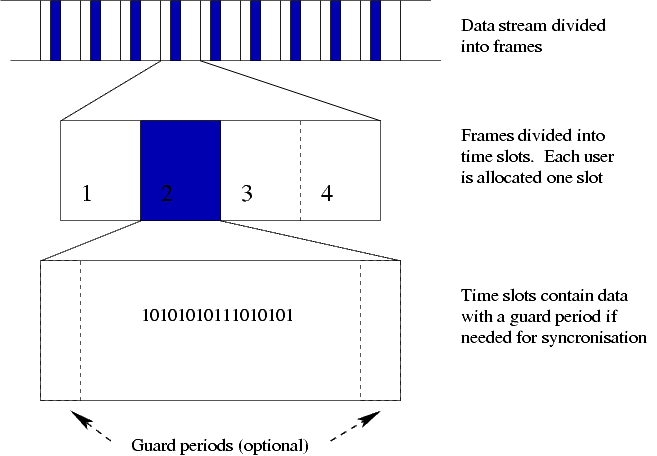
\includegraphics[width=0.8\textwidth]{assets/osi/physical/multiplexing/tdma.png}
    \caption{TDMA: Users take turns transmitting in fixed time slots}
    \label{fig:tdma}
\end{figure}

In TDMA:
\begin{itemize}
    \item The entire frequency band is available to each user
    \item Time is divided into fixed slots (called a "frame")
    \item Each user gets one slot per frame
    \item If a user has nothing to send, their slot remains empty
\end{itemize}


\subsubsection{FDMA}
FDMA has multiple dedicated perceptual "lanes" that users can occupy called channels. This is like FM radio, WiFi or even cable TV, where each channel is a separate frequency band.

\begin{figure}[h]
    \centering
    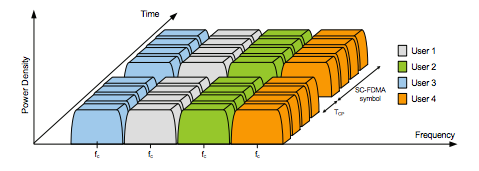
\includegraphics[width=0.8\textwidth]{assets/osi/physical/multiplexing/fdma-sc.png}
    \caption{FDMA: Users transmit simultaneously on different frequency bands}
    \label{fig:fdma}
\end{figure}

In FDMA:
\begin{itemize}
    \item Each user gets a dedicated frequency band (channel)
    \item All users can transmit simultaneously
    \item Guard bands separate channels to prevent interference
    \item Users can transmit whenever they want within their assigned frequency
\end{itemize}

Modern systems often combine these techniques! For example:
\begin{itemize}
    \item \textbf{4G LTE}: Uses both FDMA (different frequency carriers) and TDMA (time slots within each carrier)
    \item \textbf{Wi-Fi}: Uses FDMA (different channels) plus collision avoidance protocols
    \item \textbf{GPS}: Uses CDMA for satellites plus FDMA for different frequency bands
\end{itemize}

\begin{importantblock}
    Remember: These are all solutions to the same fundamental problem - how do multiple users share a limited communication medium without interfering with each other? The "best" solution depends on your specific requirements for capacity, latency, complexity, and cost.
\end{importantblock}

\subsection{FDM/FDMA, TDM/TDMA?}
You might have noticed that we've been using similar terms: FDM vs FDMA and TDM vs TDMA. What's the difference?

\begin{importantblock}
    \textbf{Multiplexing} refers to combining signals from the same source, while \textbf{Multiple Access} refers to sharing resources among different devices/users.
\end{importantblock}

In practice, these terms are often used interchangeably, but understanding the conceptual difference helps clarify whether we're talking about one device managing multiple data streams or multiple devices sharing a common medium.

\subsection{Carriers and Sensing}
\label{subsec:carriers_sensing}
As you might have noticed in Figure \ref{fig:fdma}, the graph is labelled as FDMA-SC, where the SC stands for \textbf{Single Carrier}. But what is a carrier? We've also seen that word in Section \ref{sec:modulation} when we talked about modulating signals.

\begin{importantblock}
    A carrier is a signal that can be modulated to carry information. Usually a sine wave, we augment it by modulating its amplitude, frequency, or phase to encode our data (as we mentioned in Section \ref{sec:modulation}).
\end{importantblock}

Sensing is the process of detecting whether a signal is already present on a carrier frequency. This allows devices to determine if a channel is busy or available before attempting to transmit. In TDMA systems, sensing helps verify if it's the designated time slot for transmission. In FDMA systems, sensing checks whether the assigned frequency band is clear of interference.

This brings us to a perfect (in the author's opinion) segue: carrier sensing addresses collision detection, but collision handling and recovery falls under the Data Link Layer of the OSI model. You're in luck! Enter\dots
